\section{Weitere Ergebnisse und Plots für \dimcomp{0}}

{\hypersetup{linkcolor=white} 
\begin{frame}{Testszenario I: \hyperlink{0dxmax}{Nicht stetiges Potential}}
\label{0dScII}
	\centering
	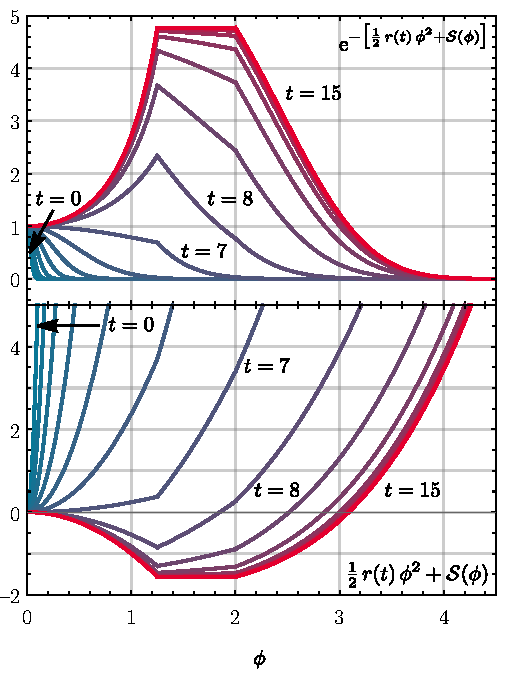
\includegraphics[width=0.47\framewidth]{../0d/figures/rg_flow_integrand_z_kink.pdf}\hspace{.5cm}
	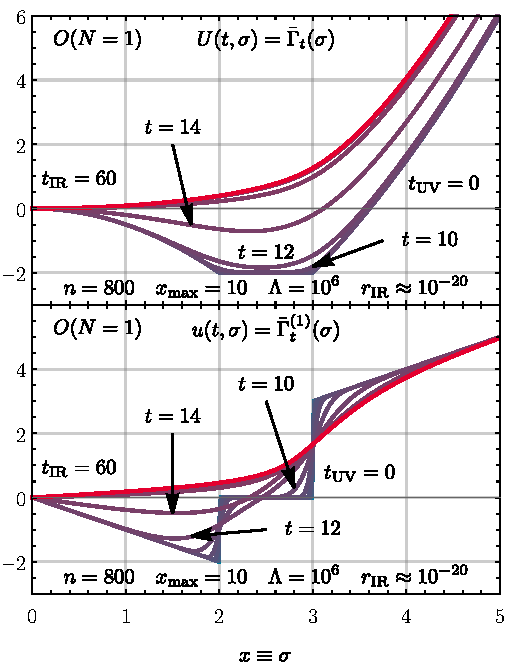
\includegraphics[width=0.47\framewidth]{../0d/figures/sc_i_on=1_n=800_xmax=10_lambda=1.0e6_tir=60_rg_flow.pdf}
\end{frame}
}

\begin{frame}{Advektion vs. Diffusion -- Pionen vs. Sigma}
	\label{0dadvection}
	\centering
	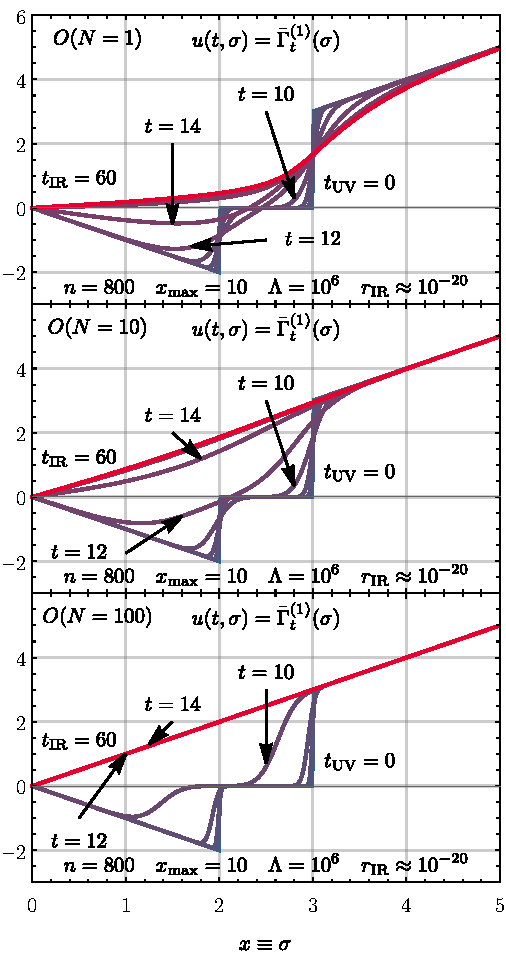
\includegraphics[width=0.38\framewidth]{../0d/figures/sc_i_on_1_10_100_n_800_xmax_10_lambda_1e6_tir_60_rg_flow.pdf}
\end{frame}

\begin{frame}{Räumlicher Diskretisierungsfehler für $	U ( \vec{\varphi} \vts ) = -\tfrac{1}{2} \, \vec{\varphi}^{\vts 2} + \tfrac{1}{4!} \, ( \vec{\varphi}^{\vts 2} )^2 $}
	\label{0dscaling}
	\centering
	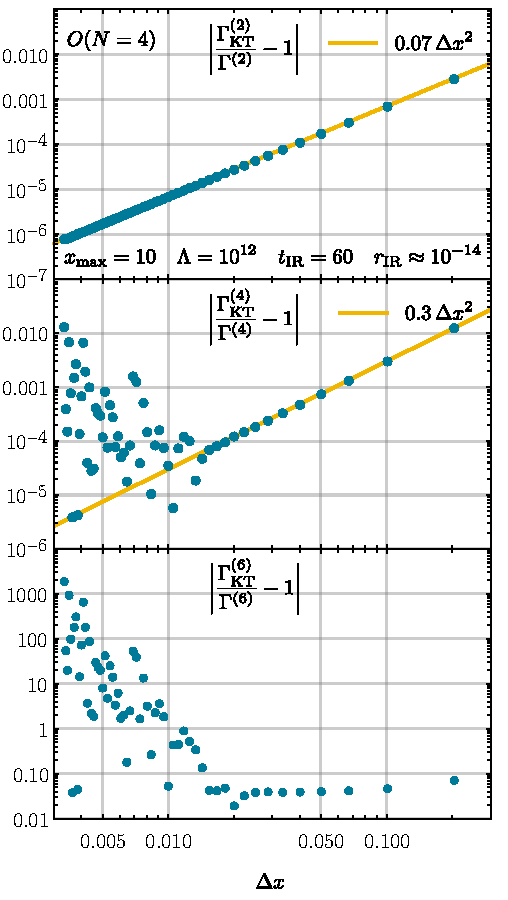
\includegraphics[width=0.38\framewidth]{../0d/figures/sc_ii_n_on_4_xmax_10_lambda_1e12_tir_60_deltax_scaling.pdf} 
\end{frame}

\begin{frame}{Berechnungsintervall für Testszenario I}
\label{0dxmax}
	\centering
	\begin{align*}
		U ( \vec{\varphi} \vts ) =
		\begin{cases}
			- \tfrac{1}{2} \, \vec{\varphi}^{\vts 2} \, ,			&	\text{if} \quad |\vec{\varphi}| \leq 2 \, ,\\
			- 2 \, ,									&	\text{if} \quad 2 < |\vec{\varphi}| \leq 3 \, ,\\
			+ \tfrac{1}{2} \, ( \vec{\varphi}^{\vts 2} - 13 ) \, ,	&	\text{if} \quad 3 < |\vec{\varphi}| 
		\end{cases}
	\end{align*}\vspace{0.5cm}\\
	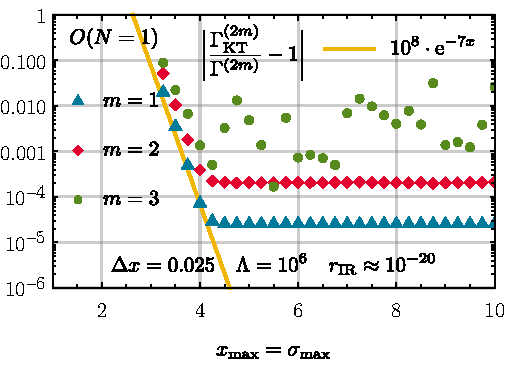
\includegraphics[width=0.47\framewidth]{../0d/figures/sc_i_on_1_deltax_25e-3_lambda_1e6_tir_60_errors_xmax.pdf}\hspace{.5cm}
	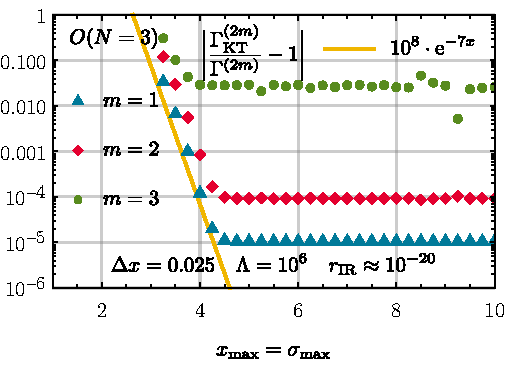
\includegraphics[width=0.47\framewidth]{../0d/figures/sc_i_on_3_deltax_25e-3_lambda_1e6_tir_60_errors_xmax.pdf} 
\end{frame}


\begin{frame}{RG-Konsistenz und UV-Skalen $\Lambda$ für Testfall I}
	\label{0dLambda}
	\centering
	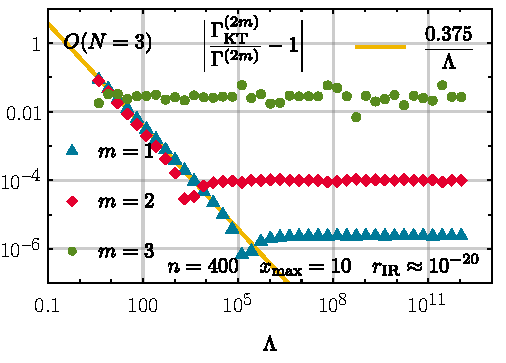
\includegraphics[width=0.6\framewidth]{../0d/figures/sc_i_on_3_n_400_xmax_10_rir_10e-20_cutoff_test.pdf}
\end{frame}


\begin{frame}{FRG Taylor-/Vertex-Expansion fürr $	U ( \vec{\varphi} \vts ) = \mp\tfrac{1}{2} \, \vec{\varphi}^{\vts 2} + \tfrac{1}{4!} \, ( \vec{\varphi}^{\vts 2} )^2 $}
	\label{0dTaylor}
	\centering
	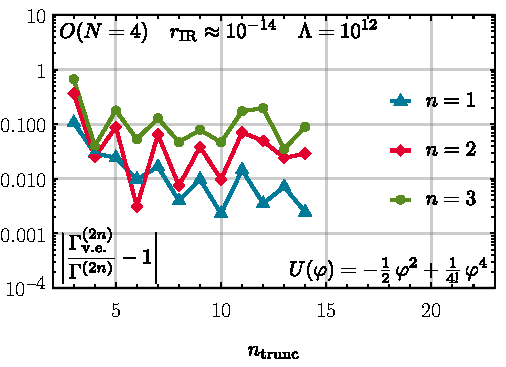
\includegraphics[width=0.47\framewidth]{../0d/figures/sc_ii_n_on_4_lambda_1e12_tir_60_vertex_exp_error.pdf}\hspace{.5cm}
	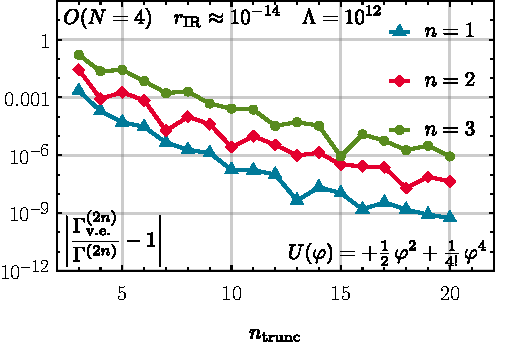
\includegraphics[width=0.47\framewidth]{../0d/figures/sc_ii_p_on_4_lambda_1e12_tir_60_vertex_exp_error.pdf} 
\end{frame}


\begin{frame}{Dynamische-Reichweite und IR Cutoffs für Testfall I}
	\label{0dkrange}
	\centering
	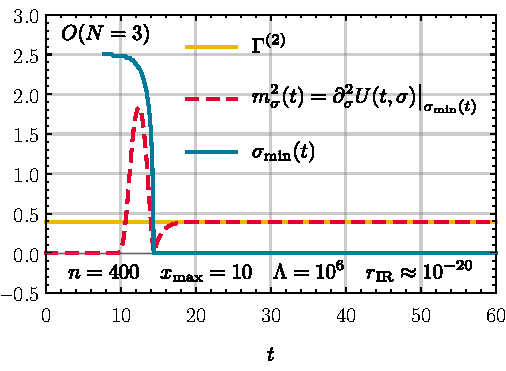
\includegraphics[width=0.47\framewidth]{../0d/figures/sc_i_on_3_n_400_xmax_10_lambda_1e6_tir_60_mass_minimum.pdf}\hspace{.5cm}
	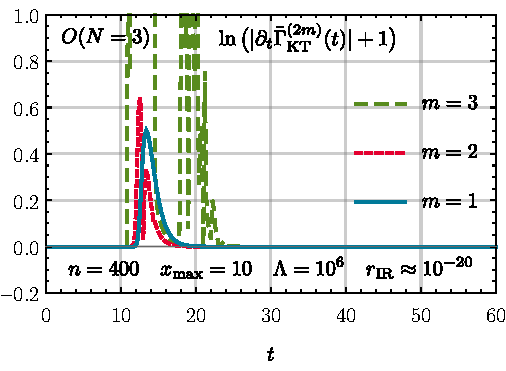
\includegraphics[width=0.47\framewidth]{../0d/figures/sc_i_on_3_n_400_xmax_10_lambda_1e6_tir_60_changing_rates.pdf} 
\end{frame}


\begin{frame}{Irreversibilität und ``Entropie''-Produktion für Testfall I}
	\label{0dentropie}
	\centering
	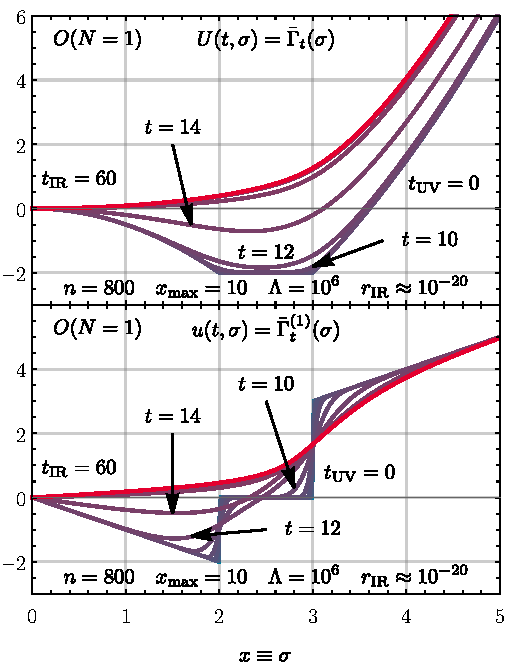
\includegraphics[width=0.47\framewidth]{../0d/figures/sc_i_on=1_n=800_xmax=10_lambda=1.0e6_tir=60_rg_flow.pdf}\hspace{.5cm}
	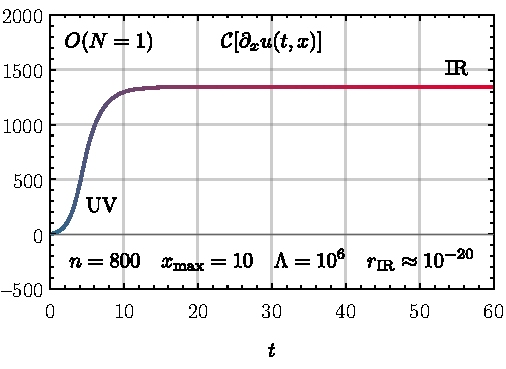
\includegraphics[width=0.47\framewidth]{../0d/figures/sc_i_on=1_n=800_xmax=10_lambda=1.0e6_tir=60_entropy_flow.pdf} 
\end{frame}


\begin{frame}{Irreversibilität und ``Entropie''-Produktion für Testfall II}
	\centering
	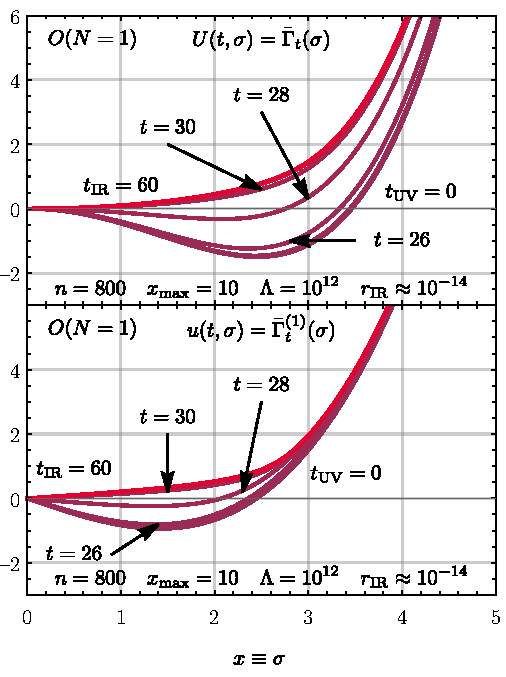
\includegraphics[width=0.47\framewidth]{../0d/figures/sc_ii_n_on=1_n=800_xmax=10_lambda=1.0e12_tir=60_rg_flow.pdf}\hspace{.5cm}
	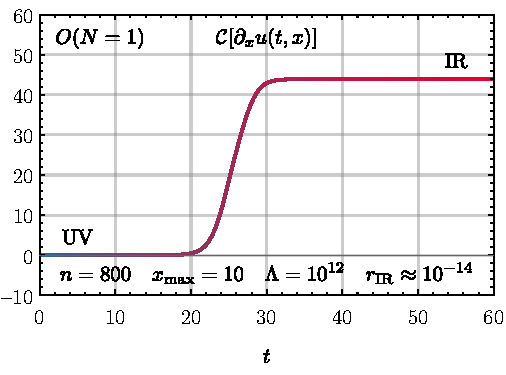
\includegraphics[width=0.47\framewidth]{../0d/figures/sc_ii_n_on=1_n=800_xmax=10_lambda=1.0e12_tir=60_entropy_flow.pdf} 
\end{frame}


\begin{frame}{Flüsse bei $N\rightarrow\infty$ und $N=32$}
	\label{0dlargeN}
	\centering
	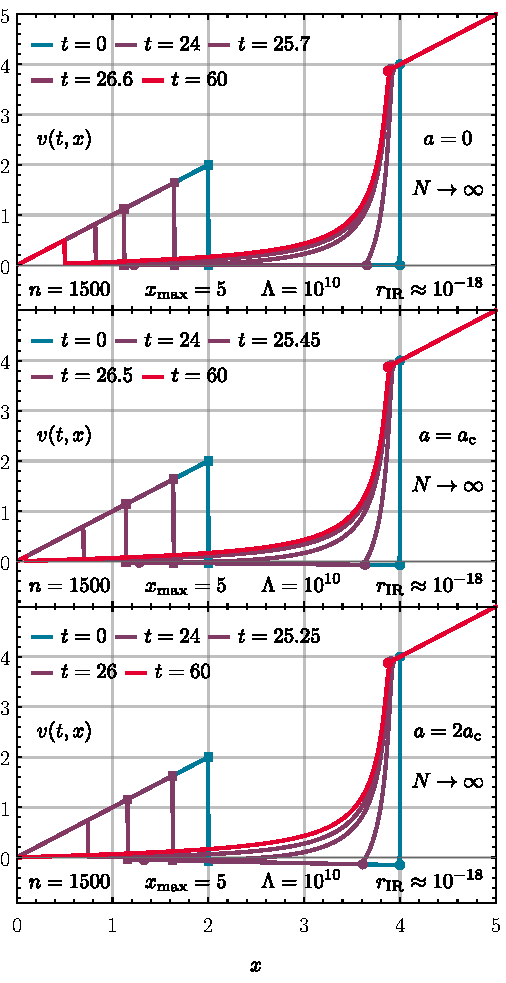
\includegraphics[width=0.36\framewidth]{../0d/figures/largeN_flows.pdf}\hspace{.5cm}
	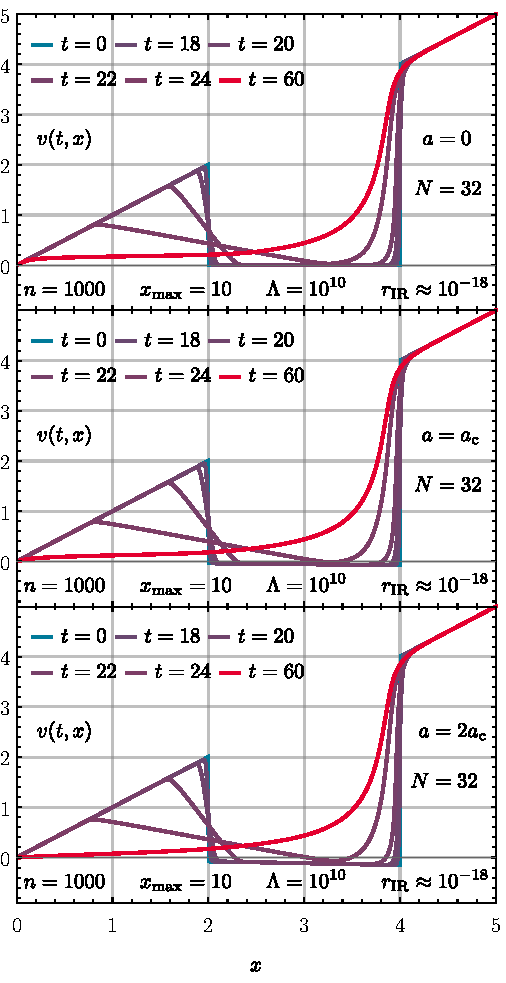
\includegraphics[width=0.36\framewidth]{../0d/figures/N32_flows.pdf} 
\end{frame}



\begin{frame}{Ein \SU{2} Model -- stark gekoppelte Graßmannzahlen}
	\label{0dfermion}
	\centering

	\begin{align*}
		\FSeaa_\FSk[\MFchi]&=\del{\MFvtx{m}{\MFrho}\suIItij{0}{\alpha}{\beta}
		+\iu \MFvtx{h}{\MFrho}\suIItij{i}{\alpha}{\beta}\MFphi_i}\MFthetab_\alpha\MFtheta^\beta+\\
		&\qquad \qquad \qquad +\tfrac{1}{2}\MFvtx{g}{\MFrho}\suIItij{0}{\alpha}{\beta}\suIItij{0}{\delta}{\gamma}\MFthetab_\alpha\MFtheta^\beta\MFthetab_\delta\MFtheta^\gamma
		+ U_t(\MFrho)
	\end{align*}
\end{frame}
